\documentclass[a4paper]{aiaa-tc}
\usepackage{xcolor}
\usepackage{graphicx}
\usepackage{titlesec}
\usepackage{verbatim}
\usepackage{amsmath}
\usepackage{mathtools}
\usepackage{listings}
\usepackage{gensymb}
\usepackage[section, above, below]{placeins}
\usepackage{caption}
\usepackage{subcaption}
\usepackage{setspace}
\usepackage{float}
\restylefloat{table}
\usepackage{tcolorbox}
\usepackage{color}
\definecolor{mygreen}{RGB}{28,172,0} 
\definecolor{mylilas}{RGB}{170,55,241}
\usepackage{mathdesign}
\usepackage{pxfonts}
\usepackage{bm}
\usepackage{wasysym}
%\usepackage{tocbibind}
\cfoot{\footnotesize\normalfont\thepage\ of \pageref{LastPage}\\\rule[.2\baselineskip]{0.5in}{0.2pt} \\ ASEN 5044 - Statistical Estimation for Dynamical Systems}
% Move table captions to above
\floatstyle{plaintop}
\restylefloat{table}
\newcommand{\volume}{\mathop{\ooalign{\hfil$V$\hfil\cr\kern0.08em--\hfil\cr}}\nolimits}
\raggedbottom
\lstset{language=Matlab,%
    %basicstyle=\color{red},
    breaklines=true,%
    morekeywords={matlab2tikz},
    keywordstyle=\color{blue},%
    morekeywords=[2]{1}, keywordstyle=[2]{\color{black}},
    identifierstyle=\color{black},%
    stringstyle=\color{mylilas},
    commentstyle=\color{mygreen},%
    showstringspaces=false,%without this there will be a symbol in the places where there is a space
    numbers=left,%
    numberstyle={\tiny \color{black}},% size of the numbers
    numbersep=9pt, % this defines how far the numbers are from the text
    emph=[1]{for,end,break,switch,case},emphstyle=[1]\color{blue}, %some words to emphasise
    %emph=[2]{word1,word2}, emphstyle=[2]{style},  
    } 

%\hspace{3.5ex}

% \begin{align*}
% \end{align*}

%\begin{equation}
%\label{e:Kinetic}
%    T = KE = \frac{1}{2}mv^2
%\end{equation}

% \begin{figure}
% \centering
% \includegraphics[width=0.91\textwidth]{Figures/OmThetaUnC.png}
% \caption{}
%  \label{fig:Name}
% \end{figure}

%\begin{figure}
%\centering
%  \begin{subfigure}[b]{0.45\textwidth}
%    \includegraphics[width=\textwidth]{Figures/Valley.png}
    %\caption{}
%  \end{subfigure}
%  ~
%  \begin{subfigure}[b]{0.45\textwidth}
%    \includegraphics[width=\textwidth]{Figures/ValleyA.png}
    %\caption{}
%  \end{subfigure}
%  \caption{}
%  \label{fig:Name}
%\end{figure}

%\begin{table}[H]
%\centering % here
%\par
%\begin{tabular}{|c|c|c|}%{\textwidth}{ |X|X|X| }
%\hline
%\multicolumn{3}{|c|}{\textbf{Error Analysis - $c_{l}$}} \\
%\hline
%\textbf{Error, \%} & \textbf{$N$ value} & \textbf{$c_{l}$}  \\
%\hline
%5 & 47 & 1.0251
% \\
%\hline
%1 & 168 & 1.0670
%\\
%\hline
%0.1 & 975 & 1.0766
%\\
%\hline
%\end{tabular}
%\caption{Results using $Error Analysis.m$ on the true $c_{l}$ value}
%\label{table:error}
%\end{table}


\title{Chris Chamberlain and Mitchell Smith \\ ASEN 5044 - Statistical Estimation for Dynamical Systems \\ Orbit Determination \\ \today}

\begin{document}
%\begin{titlepage}
    \maketitle
%\end{titlepage}

%\vspace{-1cm}
\section*{Part II -- Linearized Kalman Filter}
 \begin{figure}[H]
 \centering
 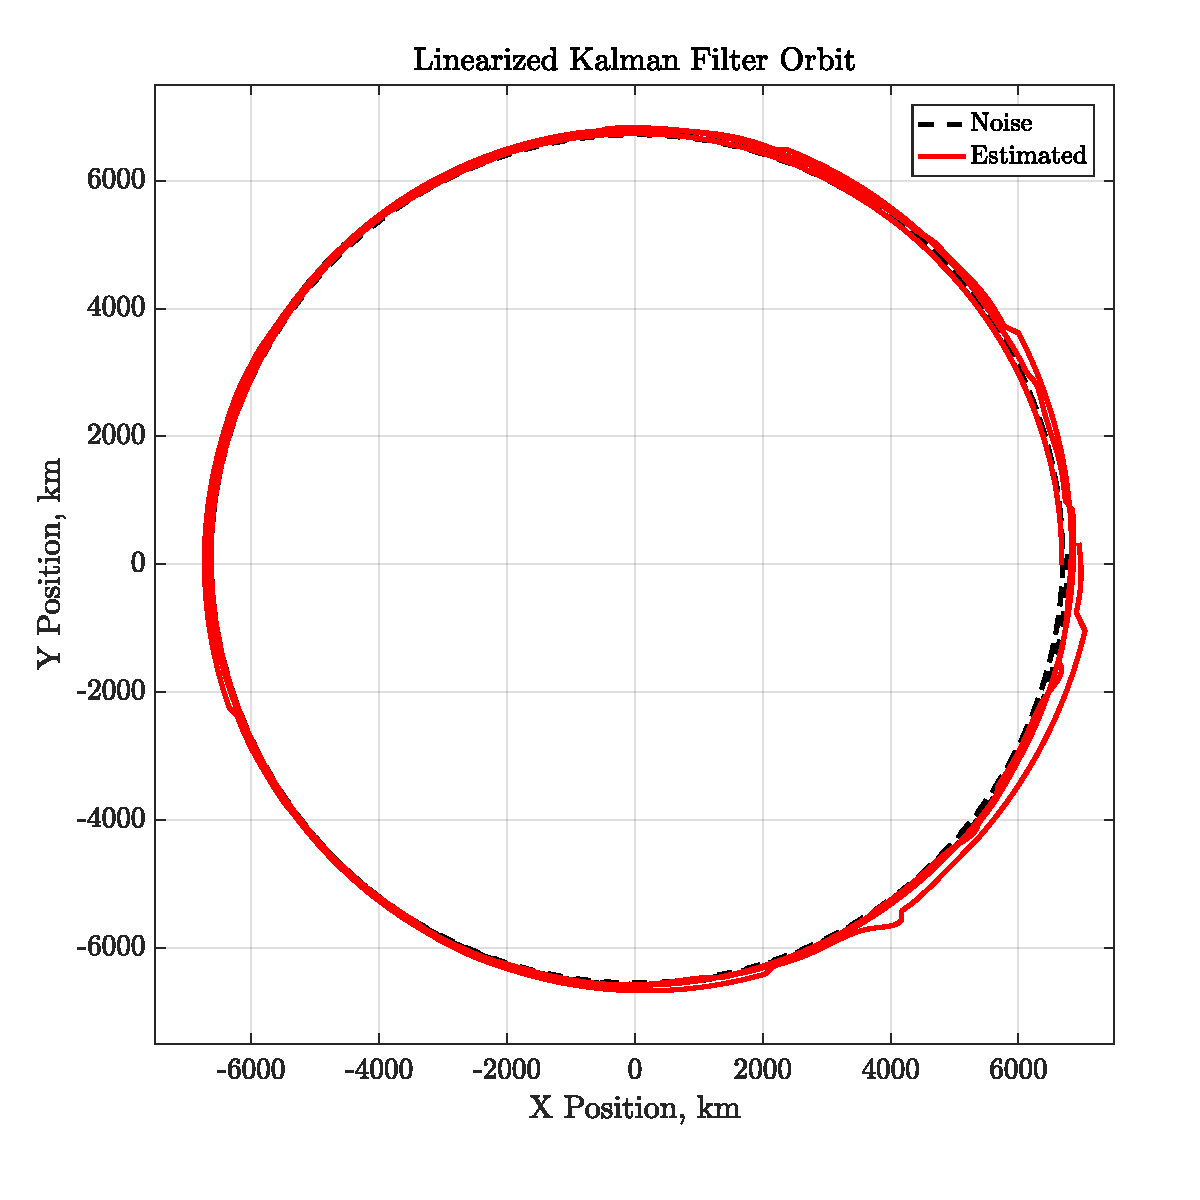
\includegraphics[width=\textwidth]{Figures/LKF_orbit.pdf}
 \end{figure}
 
  \begin{figure}[H]
 \centering
 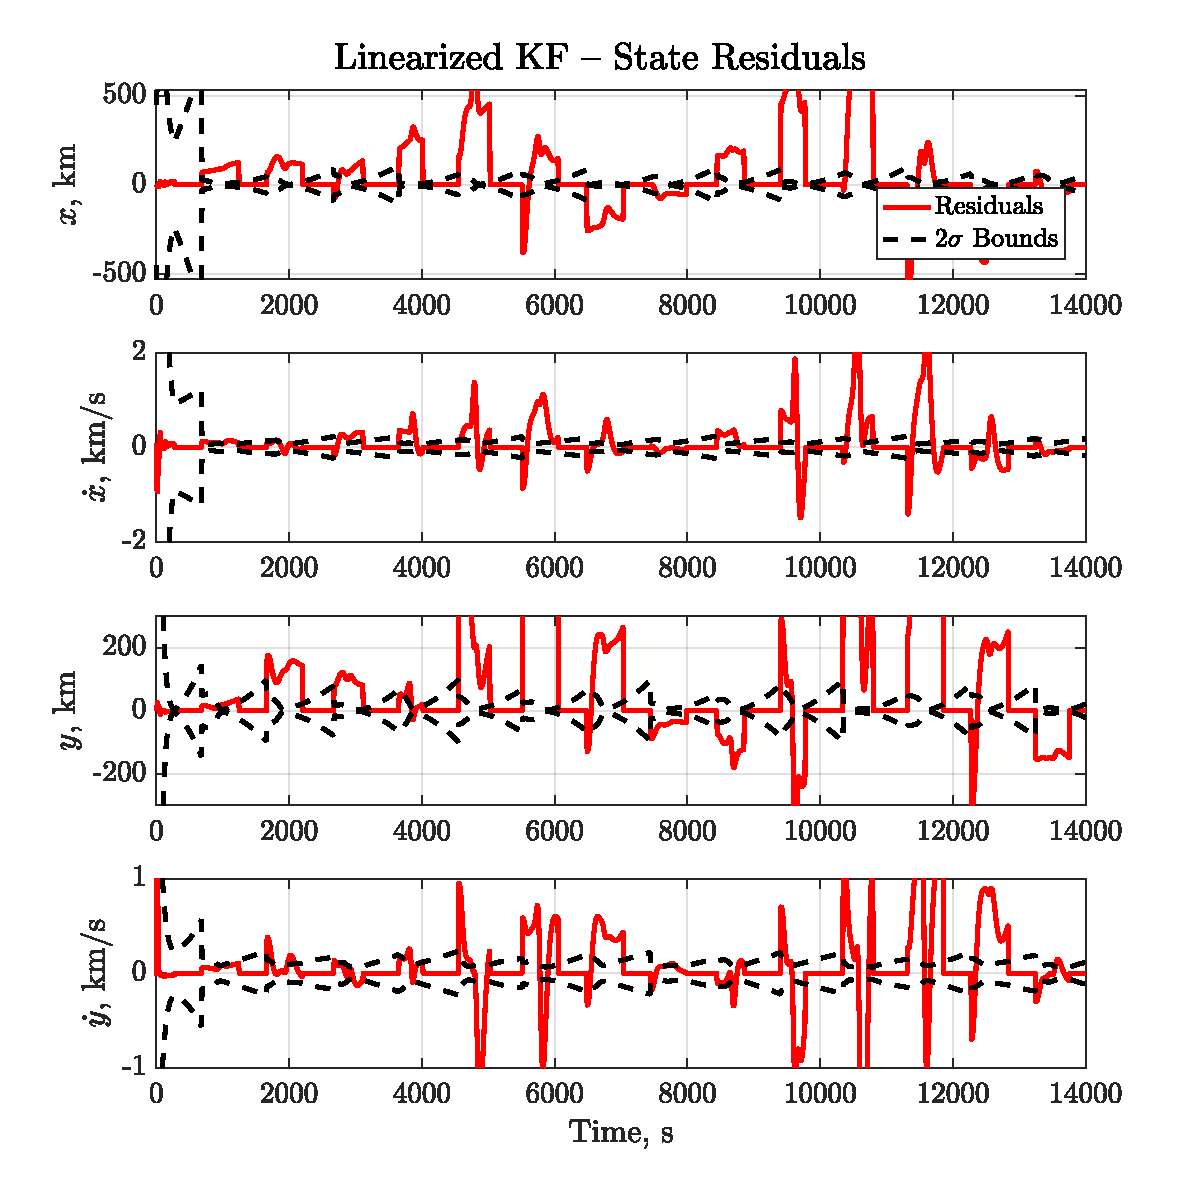
\includegraphics[width=\textwidth]{Figures/LKF_residuals.pdf}
 \end{figure}
 
  \begin{figure}[H]
 \centering
 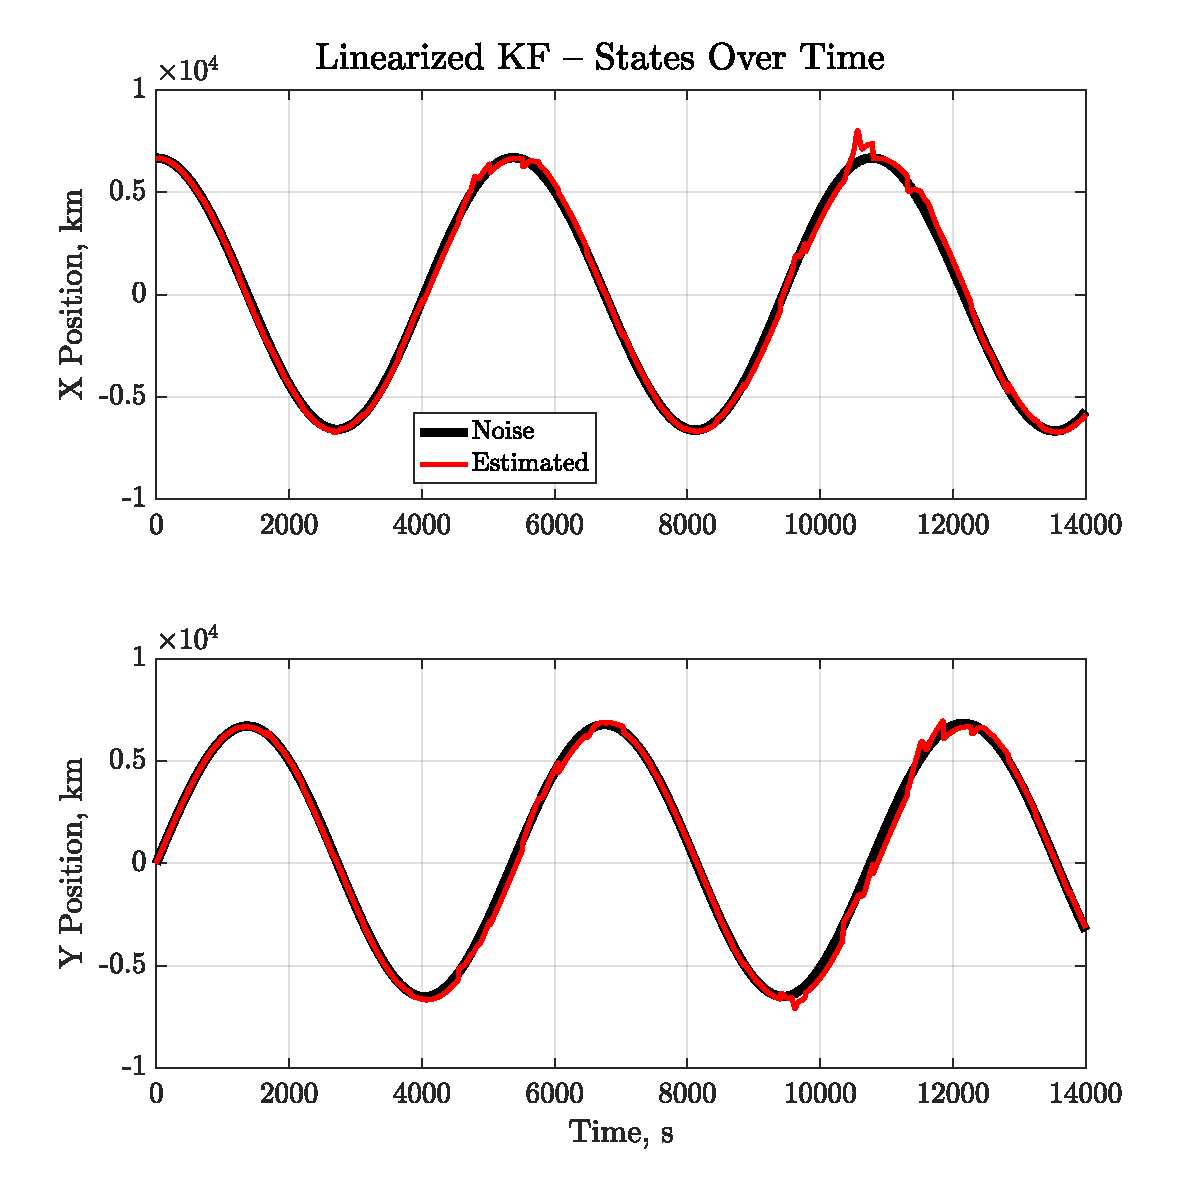
\includegraphics[width=\textwidth]{Figures/LKF_states.pdf}
 \end{figure}
 
  \begin{figure}[H]
 \centering
 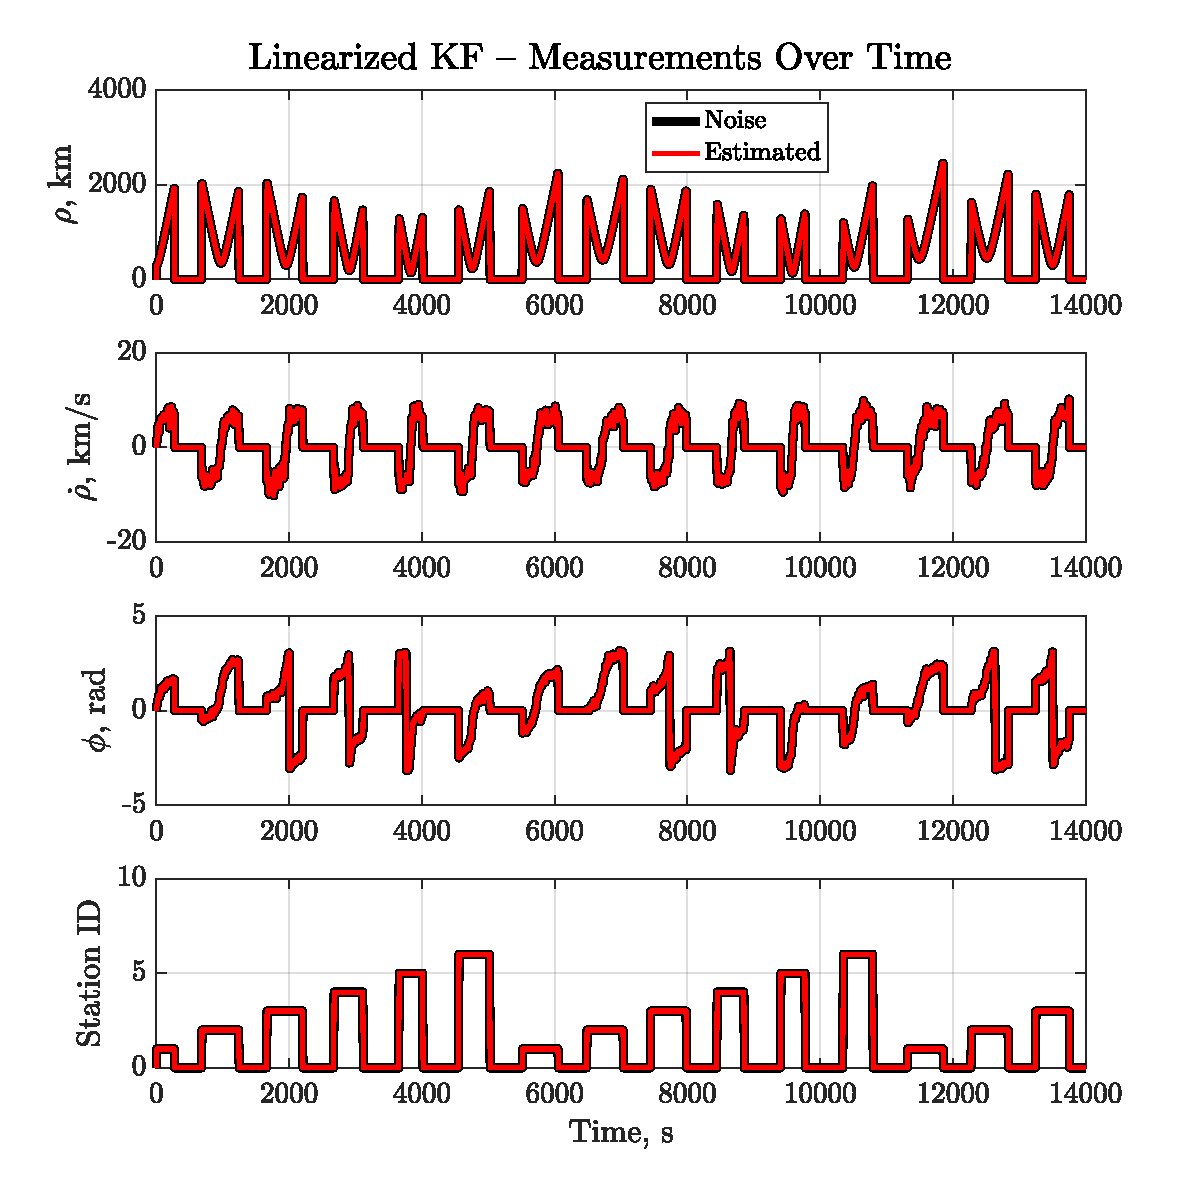
\includegraphics[width=\textwidth]{Figures/LKF_measurements.pdf}
 \end{figure}
 
  \begin{figure}[H]
 \centering
 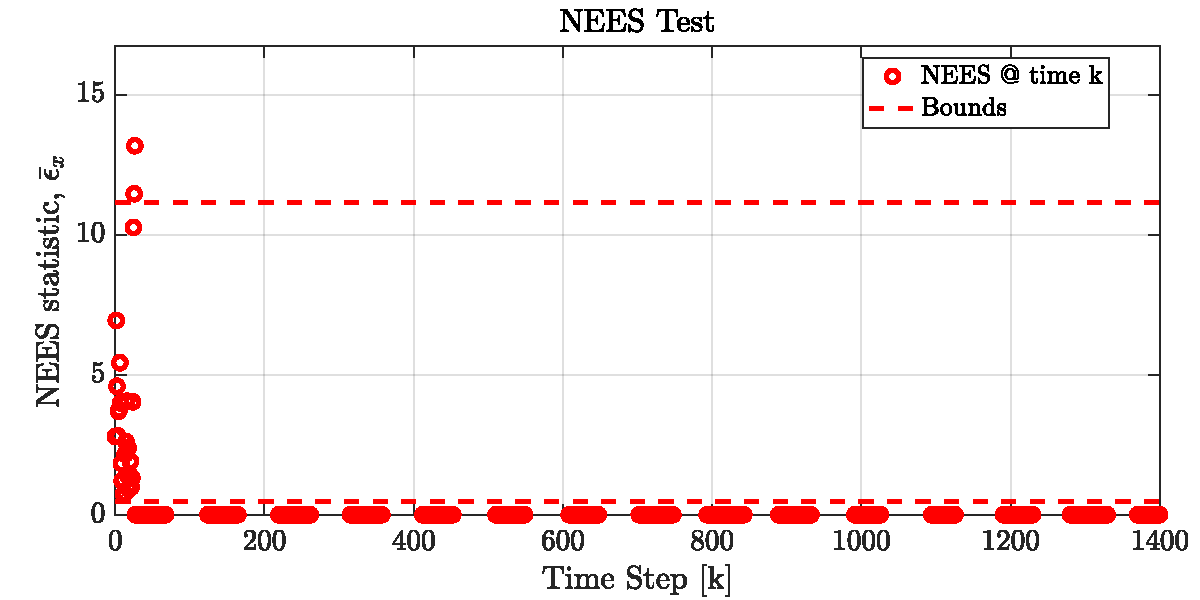
\includegraphics[width=\textwidth]{Figures/LKF_NEES.pdf}
 \end{figure}
 
 
 \section*{Part III -- Extended Kalman Filter}
  \begin{figure}[H]
 \centering
 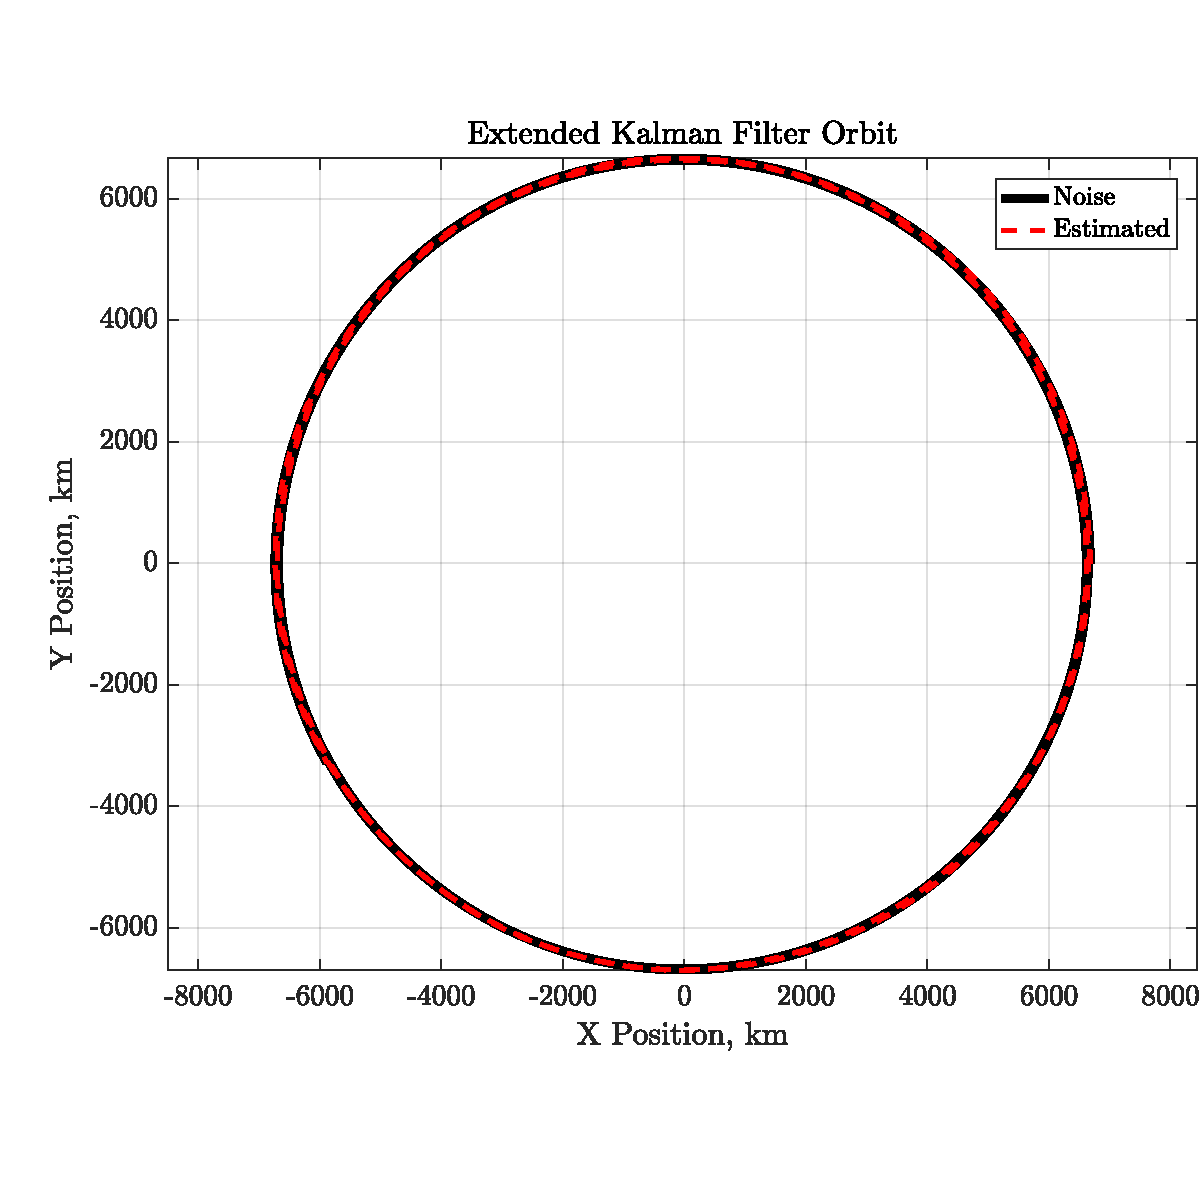
\includegraphics[width=\textwidth]{Figures/EKF_orbit.pdf}
 \end{figure}
 
  \begin{figure}[H]
 \centering
 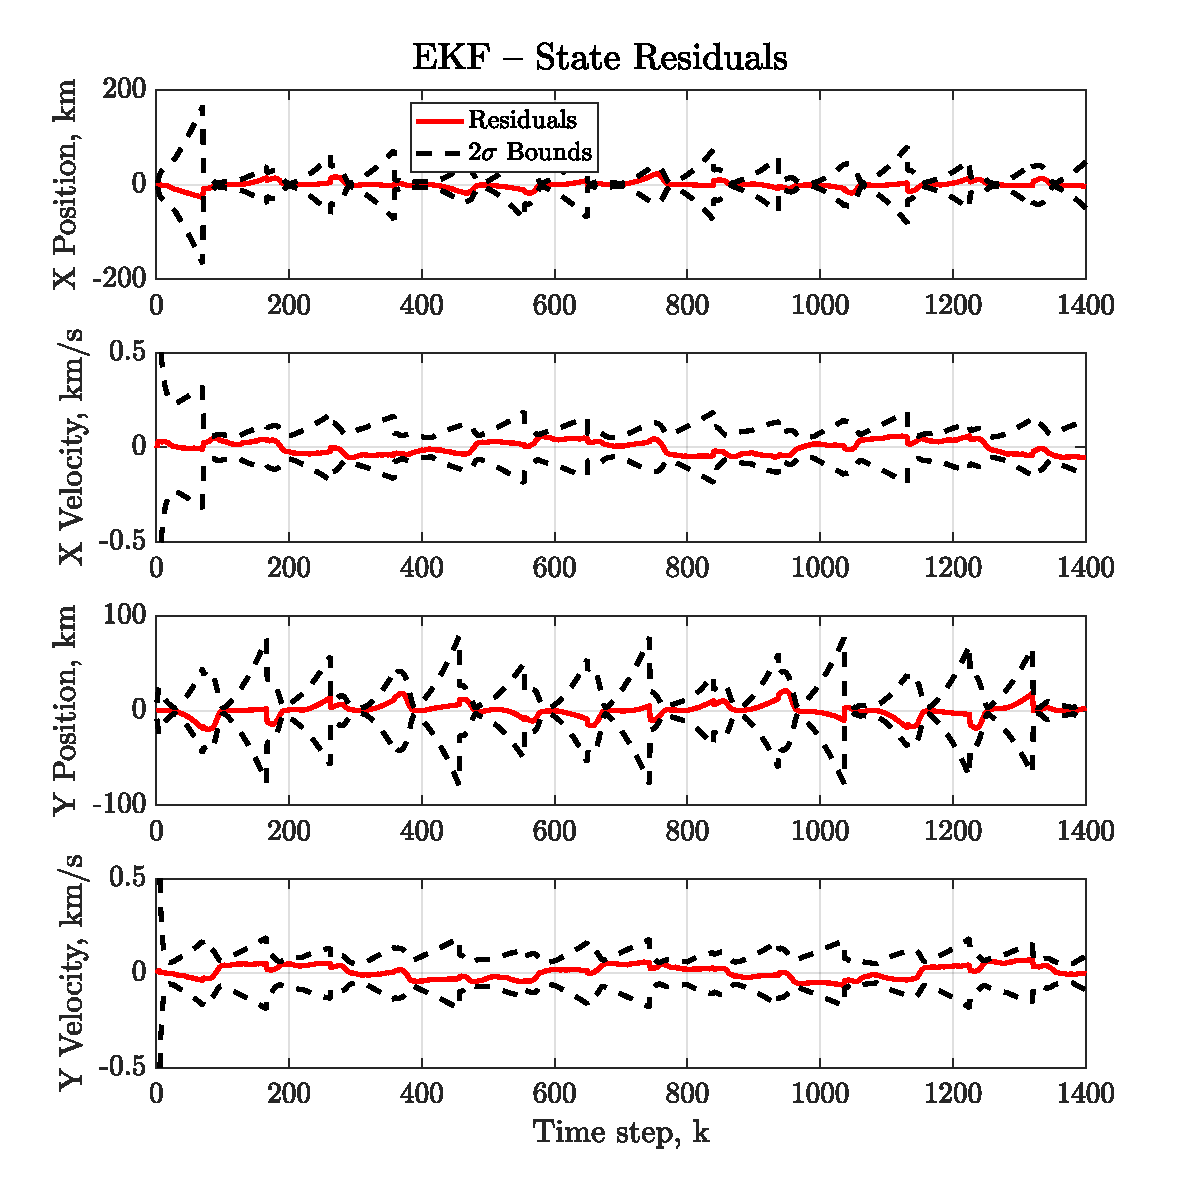
\includegraphics[width=\textwidth]{Figures/EKF_residuals.pdf}
 \end{figure}
 
  \begin{figure}[H]
 \centering
 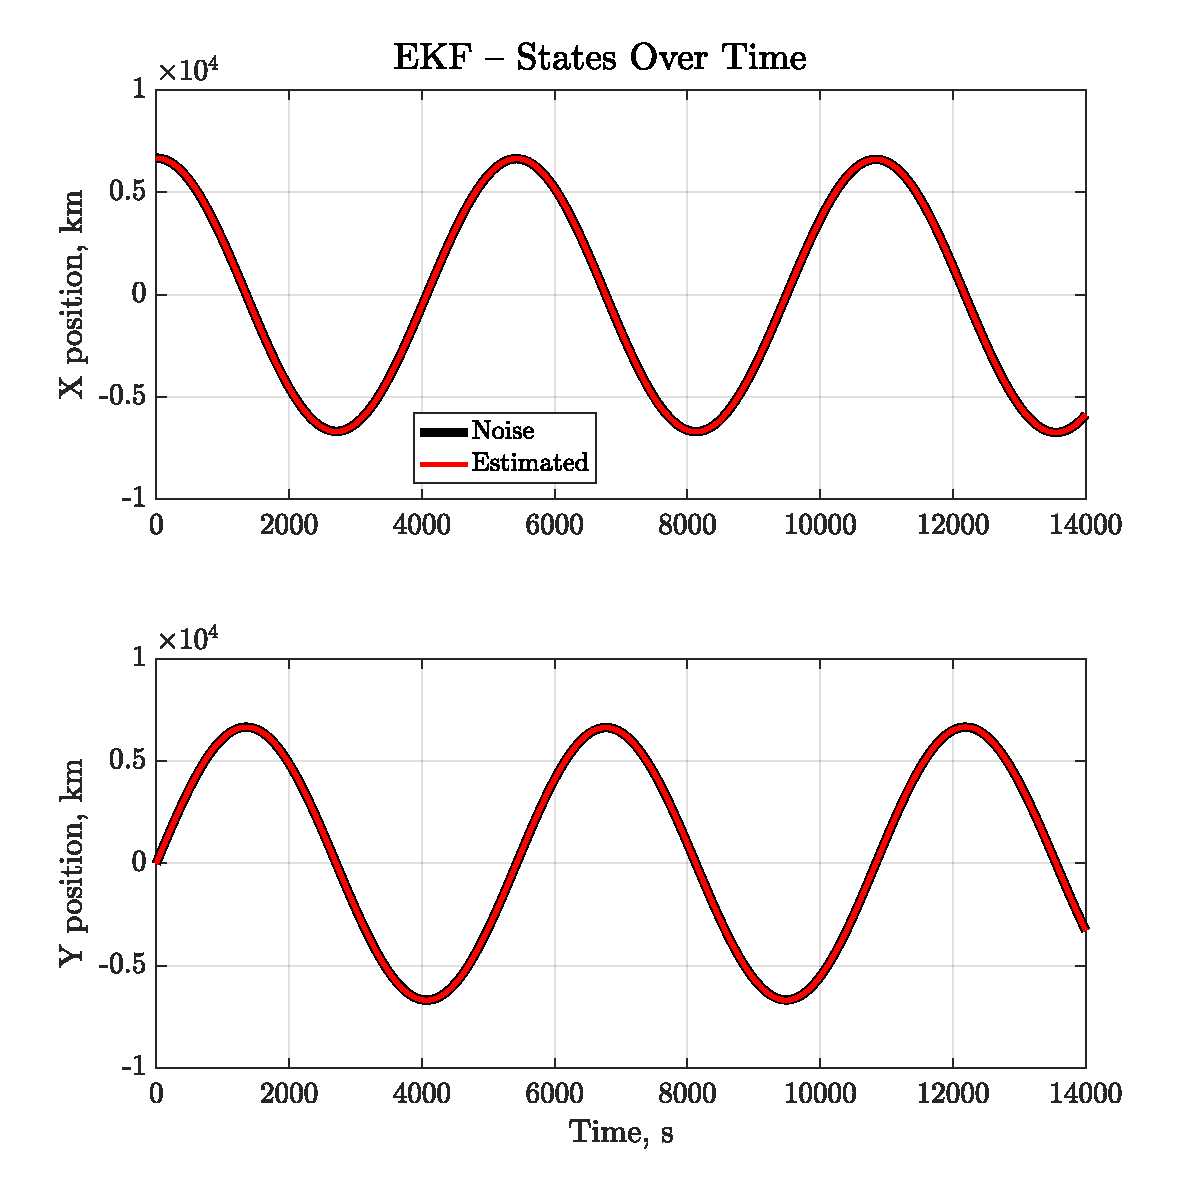
\includegraphics[width=\textwidth]{Figures/EKF_states.pdf}
 \end{figure}
 
  \begin{figure}[H]
 \centering
 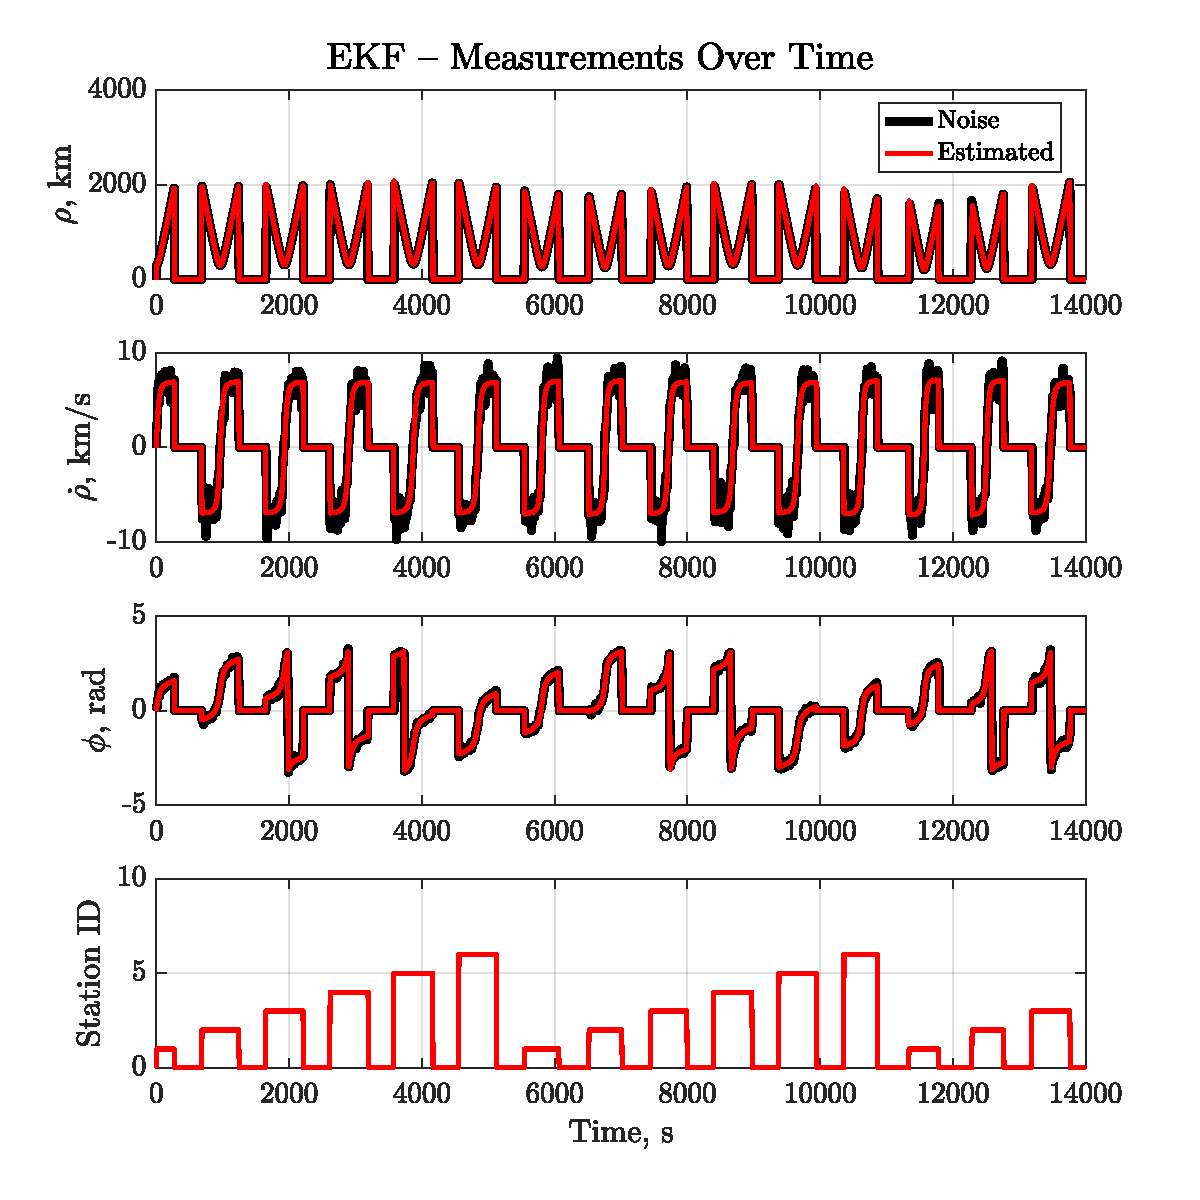
\includegraphics[width=\textwidth]{Figures/EKF_measurements.pdf}
 \end{figure}
 
  \begin{figure}[H]
 \centering
 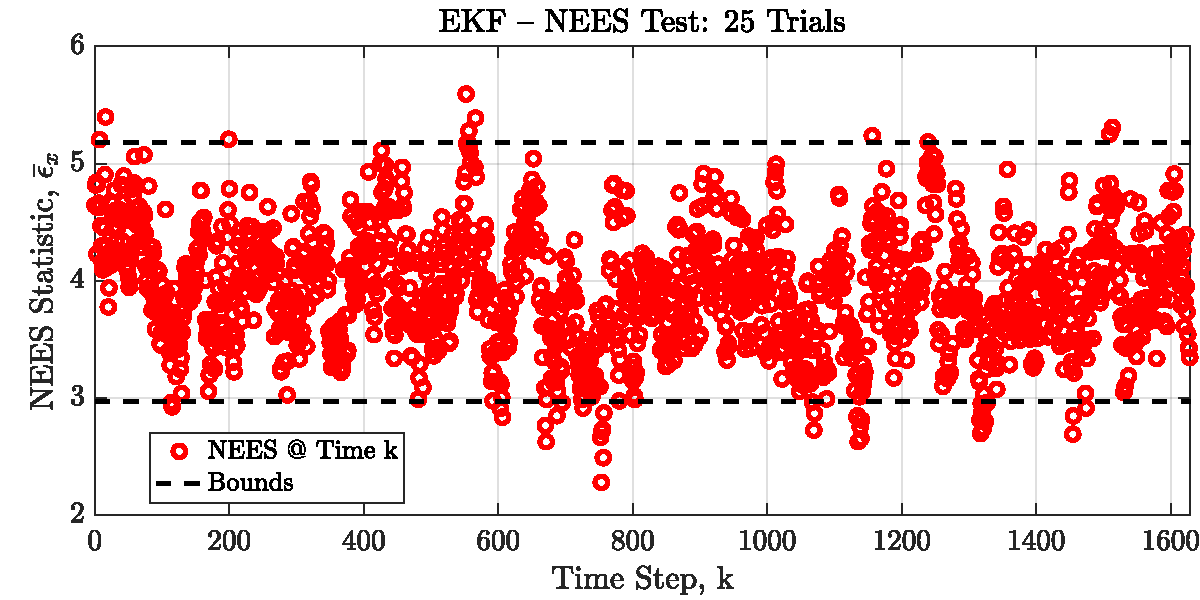
\includegraphics[width=\textwidth]{Figures/EKF_NEES.pdf}
 \end{figure}
 
  \begin{figure}[H]
 \centering
 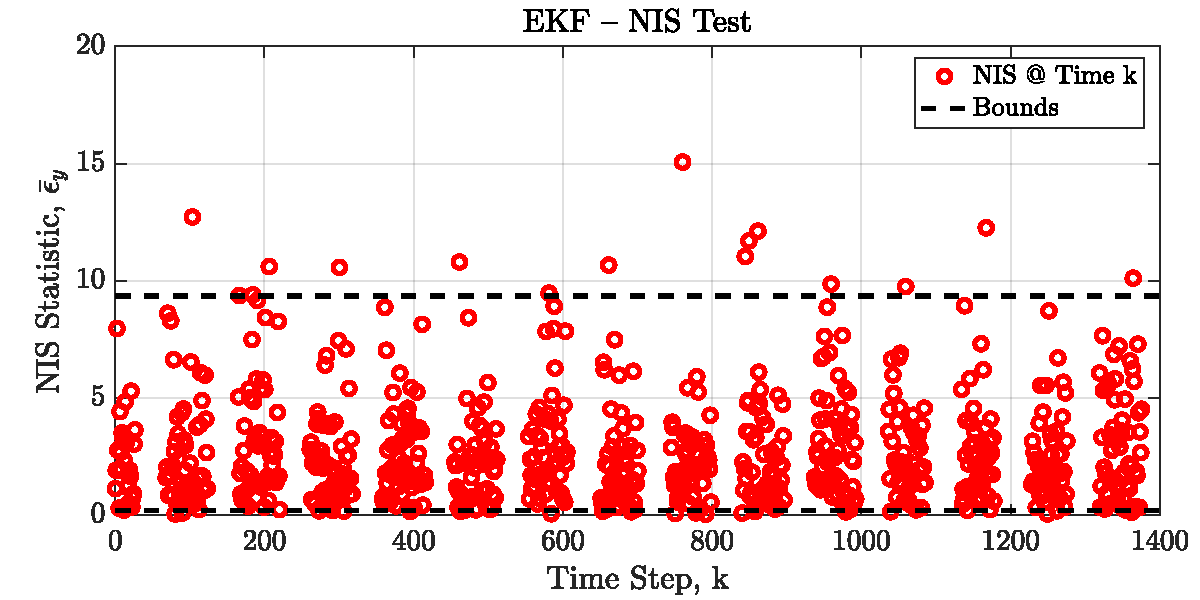
\includegraphics[width=\textwidth]{Figures/EKF_NIS.pdf}
 \end{figure}
 


%\pagebreak
%\section{MATLAB Code}
%\subsection{Main Function}
%	\footnotesize{\lstinputlisting{StatDS_HW04.m}}
%\subsection{geoidHeight.m}
%	\footnotesize{\lstinputlisting{geoidHeight.m}}	
%\subsection{gravityAnomaly.m}
%	\footnotesize{\lstinputlisting{gravityAnomaly.m}}
%\subsection{degreeVariance.m}
%	\footnotesize{\lstinputlisting{degreeVariance.m}}
%\subsection{two\_body\_ode.m}
%	\footnotesize{\lstinputlisting{two_body_ode.m}}					
	
	
\end{document}